% adapted by WS from SSR's Word document and from the 5-part series at
% https://www.overleaf.com/learn/latex/How_to_Write_a_Thesis_in_LaTeX_(Part_1):_Basic_Structure
% reviewed by MAM

\documentclass[12pt,twosided]{report}

\usepackage[titletoc]{appendix} % for adding appendix to TOC
\usepackage{biblatex}  % reference management
\usepackage{geometry}  % better margins and margin control
\usepackage{graphicx}  % to include figures
\usepackage{hyperref}  % internal and external links
\usepackage[utf8]{inputenc}  % support for non-ASCII characters
\usepackage{listings}  % typset code
\usepackage{outlines}  % easy nesting of lists
\usepackage{tabularx}  % more control over table column width
\usepackage{titlesec}  % customize chapter title 
\usepackage{upquote}  % prevent mishandling of single quotes in listings


% TODO: Customize the appearance of hyperref links using \hypersetup
% See https://en.wikibooks.org/wiki/LaTeX/Hyperlinks#Customization

% Custom format of chapter title.
\titleformat{\chapter}[hang]{\bf\huge}{\thechapter.}{2pc}{}

% Separate folder for images named 'images'.
\graphicspath{ {images/} }

% Separate file for references
\addbibresource{references.bib}

% Replace with your title
\title{Project Cleanup}

% Allow recalling document title
% from https://tex.stackexchange.com/a/15806/44301
\makeatletter\let\Title\@title\makeatother  

\begin{document}

\begin{titlepage}
  
  \newgeometry{top=100pt,bottom=75pt}   
  \begin{center}
    \vfill
    \textbf{\Huge \Title}
    \bigskip

    {\large Kaavish Report\\
      presented to the academic faculty\\
      by\\\bigskip
      \begin{tabular}{ll}
        Muhammad Tahir & mt02264\\
        Muhammad Ahsan Syed & ms02743\\
        Zoha Salani & zs02816\\
        Ashhar Ayaz & aa02200\\
      \end{tabular}
    }\\\vfill
    \includegraphics[width=.4\textwidth]{logo.pdf}\\
    {\large In partial fulfillment of the requirements for\\
      \textit{Bachelor of Science}\\
      Computer Science\\\medskip
      \textbf{Dhanani School of Science and Engineering}\\\medskip
      Habib University\\\smallskip
      Spring 2020
    }\\\vfill
    Copyright {\scriptsize \textcopyright} 2019 Habib University
  \end{center}
  \restoregeometry
\end{titlepage}

%%% Local Variables:
%%% mode: latex
%%% TeX-master: "report"
%%% End:
  % title page.
\include{approval}  % approval page.

\chapter*{Dedication}
For ammi, abbu, and pappu.

\chapter*{Acknowledgements}
We want to thank the CS faculty and ...

\chapter*{Abstract}
Abstract goes here

% The following are automatically populated by LaTeX \chapter, \section and related, \figure, and \table.
\tableofcontents
\listoffigures
\listoftables

% TODO: Put chapters in a separate folder named 'chapters'.

\chapter{Introduction}
\label{chap:intro}
\section{Problem Statement}
Karachi, the city home to 21.2 million people is amidst a “Garbage Crisis”, a crisis that continues to pollute the city effecting the health and safety of millions of people. It is ranked to be the 134th in a list of 140 cities as the world’s least livable cities. It is Crisis, a problem which requires immediate attention.\\
\\
The garbage crisis encompasses lifting the garbage up as well as disposing it off and not dumping it on any piece of land. The ongoing situation of trash is such that people are dumping trash wherever they find heaps of trash and no adequate measures are being taken in order to clean those spots. The crises seems to have no end in sight as each government has made promise to clean up the economic and the financial hub of the country but none of them have been able to fulfill their commitment due to countless reasons which include lack of funds, inadequate resources and incompetence.\\
\\
Hence, in a attempt to solve a large part of this crisis we'd be addressing the problem of quantification of Garbage to aid the current resource allocation process.


\section{Proposed Solution}

We aim to build an application that is a no cost, crowd sourced solution that address the problem of quantification of garbage in a dump. In order to do this we will be using a two-step approach. The first step is to build a mobile application that allows citizens to upload images of garbage to a server. The second step then involves analysis on the image using image processing techniques in order to quantify the data.\\
\\
Now the process of quantification of data is further divided into two steps. The first step being the identification of the garbage and the second step is the quantification of it.\\
\\
The application will be able to detect and coarsely segment garbage regions in a user-clicked Geo-tagged image. It will then be processing the image, getting the location and estimate of the garbage, resulting in providing an efficient route for a garbage truck in order for it to use as less resources as possible.
A detailed description of each module of the system is presented later in Chapter ~\ref{chap:intro}.

\section{Intended User}

The intended users are the citizens of Karachi, who are tired of seeing dumps of garbage in their neighbourhood and want to contribute towards getting rid of this problem by doing their part that is taking a picture and uploading it. This would result in the authorities not only being notified but also result in them being provided with adequate information for resource allocation.

\section{Key Challenges}

Some of the key challenges faced were:\\
\\
1)Integrating of all the modules.\\
2)Familiarizing ourselves with cloud computing which was a fairly new domain for us to explore.\\
3)Free and limited trials for additional modules.\\
4)Making the flow of the final product as smooth as possible and minimizing the processing delay.\\
5)Working with Android Studio as a framework for the application development.


\chapter{Literature Review}
\label{chap:lit}
Waste management is one of the most important issue in any country of the world. If not managed properly, it can threat the health and welfare of the general population.\\
\\
The key players that are responsible for the management of solid waste are the local governments of cities and provinces/states that handle this issue. The secondary players are Non-Governmental Organizations that also work in order to efficiently manage and recycle waste.\\
\\
This section will explore the methods as well as the technologies that have been used to identify and quantify garbage:\\
\\
Around the globe there are multiple technological platforms that exist which help and collaborate with these governments and/or Non-Governmental Organizations. Most of these platforms just use a simple complain system. Some examples are:
\section{Example Platforms:}
\subsection{Dallas sanitation service, 1800 recycle} are technological platforms that attempt to deal with the management of garbage by focusing on collection of garbage based on receiving requests.
\subsection{Rubicon} is another application which makes it easy to request garbage pickup service on the go, for a single location or many locations \cite{rubicon}.\\
\\
Another such example is GarbageCAN which works towards creating an app through which we can receive requests to collect recyclables that will be sold off to different recycling companies in the city.\\
\\
In terms of Pakistan not much work have been done towards the quantification and identification, however, Lahore Waste Management Company has launched an app called "Clean Lahore" which is also used to register different type of complains but none of these work on image processing and path optimization \cite{rizvi}.\\
\\
The government however has struggled with resources and has never implemented technology in this process.There are also many NGO's that operate within Pakistan that work on waste management. These mostly work in smaller scales with or without government collaboration. NGO's like WasteBusters are such examples that hire private cleaners to do this job.\\
\\
Now having discussed the generic technological innovation catering to the garbage crisis, we shall now discuss the efforts towards the identification and quantification of image using the analysis of image and employing computer vision techniques.
\section{Identification:}
\subsection{SpotGarbage} 
SpotGarbage is an example of an app which detects and coarsely segments garbage regions in a user-clicked Geo-tagged image \cite{mittal}. It is an application that we have tested out and are using for the identification segment of our project.
\section{Quantification:}
\subsection{Dimension of Object:}
Quantification requires volume estimation and there are different methods to extract 2 dimensions of any object from a 2D image if we have a reference object with its known dimensions.\\
\begin{figure}[!hb]
   \centering
   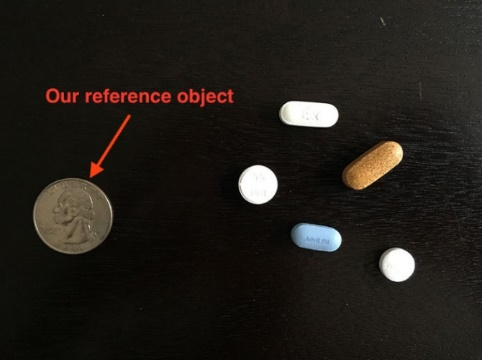
\includegraphics[scale=0.8]{images/q1.png}
   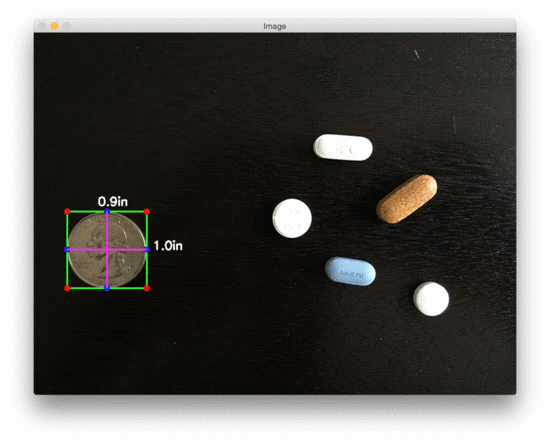
\includegraphics[scale=0.3]{images/q2.png}
   
   \caption{Dimensional Method}\label{fig:picture}
\end{figure}
\\
In the above figures there exists a reference object which is a coin whose 2 dimensions are known to us. Using that as a reference, we can calculate the dimensions of objects within the same frame. Now if another image is taken from a side angle ($90^{o}$ to the first image taken from the front angle) then we can also get 2 more dimensions. By this process we are getting the required dimensions to calculate an estimated volume of an object. However, as for the object of reference is concerned the drawback is there is a need of  reference object of known dimensions which could serve as reference for the mathematical model.
\subsection{Depth Analysis and Stereoscopic Vision:}
It uses two camera lenses, spaced slightly apart, to let the phone compare two images and piece together the depth of objects in stereo \cite{chaim}.\\
\\
The drawback of both the above mentioned techniques is that there are a lot of variables involved and that the camera particularly requires two lenses which becomes a pre-requisite for users when uploading an image to be identified or quantified but because of stereoscopic vision and depth analysis there are features that can be extracted which helps in estimating the distance between the camera and the object through which the size of the object can be estimated. \\
\\
\begin{figure}[!hb]
   \centering
   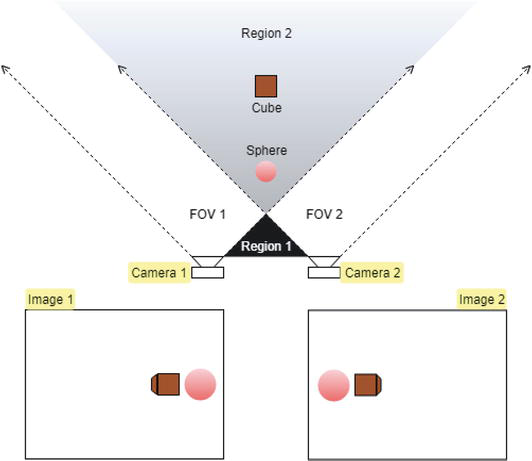
\includegraphics[scale=0.8]{images/q3.png}
   \caption{Depth Sensor/Stereoscopic Vision}\label{fig:picture}
\end{figure}
\\
This figure gives an idea of how things work. These techniques only work on stereo images from stereo cameras.
\subsection{3D Reconstruction from Multiple 2D Images:}
Another approach towards the quantification of garbage is 3D reconstruction from a single 2D image. Once we have a 3D model then the information about its volume can easily be obtained.\\
\\
Susheel, Suresh \cite{suresh} using images from 8 different perspectives were able to achieve an accuracy of 85 percent when quantifying using 3D Reconstruction. It utilized multiple 2D images from different angles on an object. Once we have those images then we can reconstruct an approximate 3D model from them.\\
\\
\begin{figure}[!hb]
   \centering
   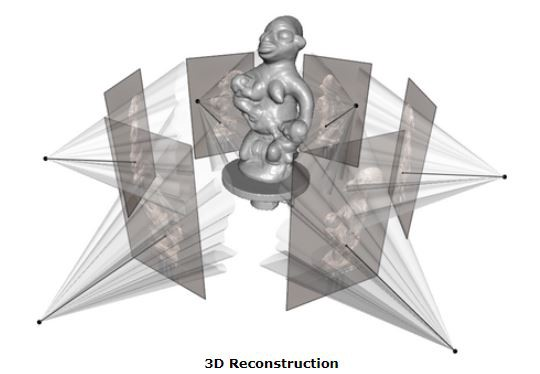
\includegraphics[scale=0.8]{images/q4.png}
   \caption{Dimensional Method}\label{fig:picture}
\end{figure}

The above mentioned figure is an example of 3D reconstruction where 6 2D images are being used.
The drawbacks of using techniques such as  3D reconstruction are 3D scanning, and the use of depth/range cameras are very costly and cumbersome to use.\\
\\
In order to improve this waste management as well as improve the communication gap present between both parties we wish to present a solution which uses images as well as locations to optimize waste collection and disposal.
\section{Object recognition}
Segmentation of garbage dumps from a scene.
Traditional approaches to segmentation, include image clustering. Image regions are clustered based on pixel intensities using an algorithm like Kmeans. This methodology would not work in our case because the region of interest (garbage dump), has varying pixel intensities in random distributions (very high spatial frequency). Also the number of clusters could not be fixed because the background would keep changing for every dump \cite{naik}\\


\chapter{Software Requirement
Specification (SRS)}
\label{chap:srs}
This chapter provides detailed specifications of the system under development.

\section{Functional Requirements}
These functions are logically grouped into modules based on their purpose/users/mode of operations etc (as per our system). \\
\\
There are three primary actors involved in this system which includes the user, the admin and the system itself so we have broken down the functionality into three modules since each module has various functional components. \\
\\
The user modules includes all the functionality that is required by the user for the system to work that is clicking various buttons in order to get the system to work. The admin model includes the functionality required by the admin to get the app to work and lastly the system module to be functional in order for the app to be functional.  
\begin{outline}
  \1 \textbf{User Module}:
  \2 Function 1: User should be able to take capture an image by clicking the button.
  \2 Function 2: User should be able to log in and out of the system.
  \2 Function 3: User should be able to sign-up into the system.
  \2 Function 4: User should be able to add the job.
  \2 Function 5: User should be able to add some description while uploading the job.
  \2 Function 6: User should be able to view the jobs he has posted.
  \1 \textbf{Admin Module}:
  \2 Function 1: Admin should be able to log in and out of the system.
  \2 Function 2: Admin should be able to view the route.
  \2 Function 3: Admin should have all control of the system including the features on all of the portals.
  \2 Function 4: Admin should be able to view all the jobs that have been posted.
  \2 Function 5: Admin should be able to add and remove other admins.
  
  \1 \textbf{System Module}:
  \2 Function 1: System should be able to take a picture.
  \2 Function 2: System should be able to upload the job in the server.
  \2 Function 3: System should be able to pre-process the images which includes data cleaning.
  \2 Function 4: System should be able to identify garbage.
  \2 Function 5: System should be able to accept and reject images on the basis of identification.
  \2 Function 6: System should be able to quantify the garbage in the image.
  \2 Function 7: System should be able to generate a route.
  \2 Function 8: System should be able to display the generated route to the admin.
\end{outline}

% --- The above is to be modified as per your project, e.g. a flat list if your system has limited functional requirements.
\newpage
\section{Non-functional Requirements}

The primary non-functional requirements that lies in our system are:\\
\\
\textbf{Accessibility}:
Accessibility is regarded as the ability to access or benefit from the system. The application will be directly/indirectly accessed and compatible with latest technology by a wide range of people. Whenever the application is accessed on any user device it should be operate-able.\\
\\
\textbf{Availability}: 
Availability is regarded as the total time an application is capable of being used during a time period. The application will be available and operate-able throughout the day with down time percent $<0.9998$.\\
\\
\textbf{Durability}: 
Durability is regarded as the application being functional without requiring any excessive maintenance and repair. The application will remain functional, without requiring excessive maintenance or repair, when faced with challenges of normal operation.\\
\\
\textbf{Integrability}: 
The application will be able to bring all sub-systems together in one single system and is able to deliver its functionality. The system will be able to coordinate will all its sub system which includes the machine learning model, database and the cloud server.\\
\\
\textbf{Maintainability}:
Maintainability is regarded as the continuous improvements of the system. The system developed should be easy to maintain. In case of any errors, it should be easy for the maintenance team to repair that error with utilizing minimum resources.\\
\\
\textbf{Reliability}:
Reliability is said to be that the system is able to function under stated conditions and for a specified period of time. Hence the system will be reliable while performing any task, it should not fail while performing the same task again. The failure ratio should be minimized.



\newpage
\section{External Interfaces}

\subsection{User Interfaces}
The Mockups are divided into two categories:\\
1- The User Panel (Mobile Application) \\
2- The Admin Panel (Web Application)\\
\\
\textbf{User Panel:}
The User Panel will provide the user with two options. They can choose to either sign in to the system using and ID and password which they previously created or sign up into the system if they are using the application for the first time. 


\begin{figure}[!hb]
   \centering
   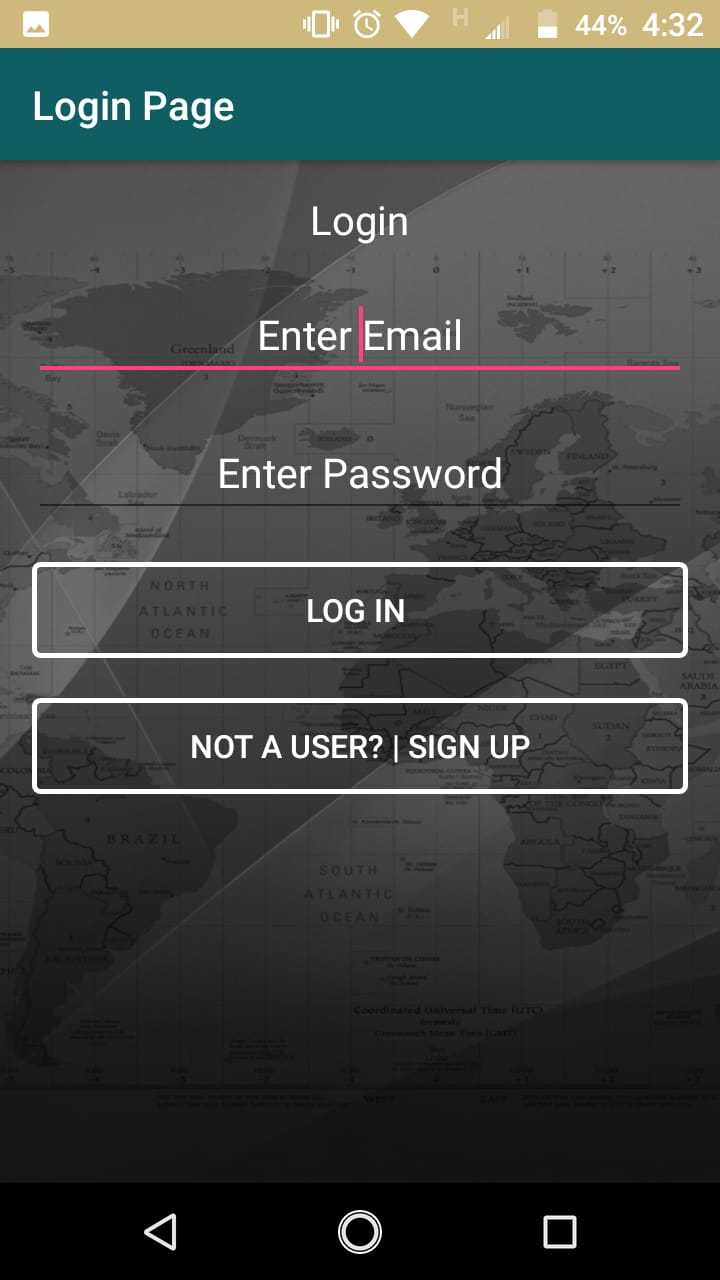
\includegraphics[scale=0.5]{images/1.png}
   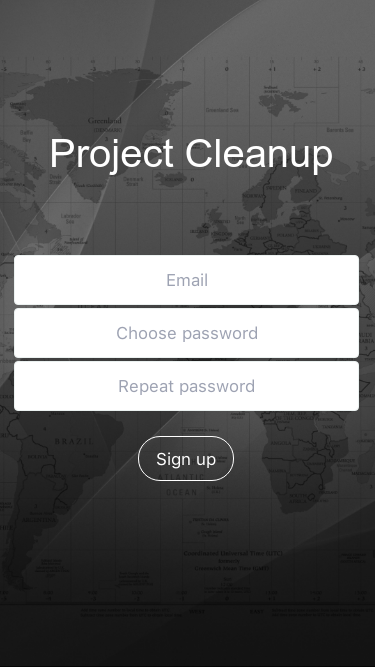
\includegraphics[scale=0.5]{images/2.png}

 
   \caption{User Panel}\label{fig:picture}
\end{figure}
\newpage
\begin{figure}[!hb]
   \centering

   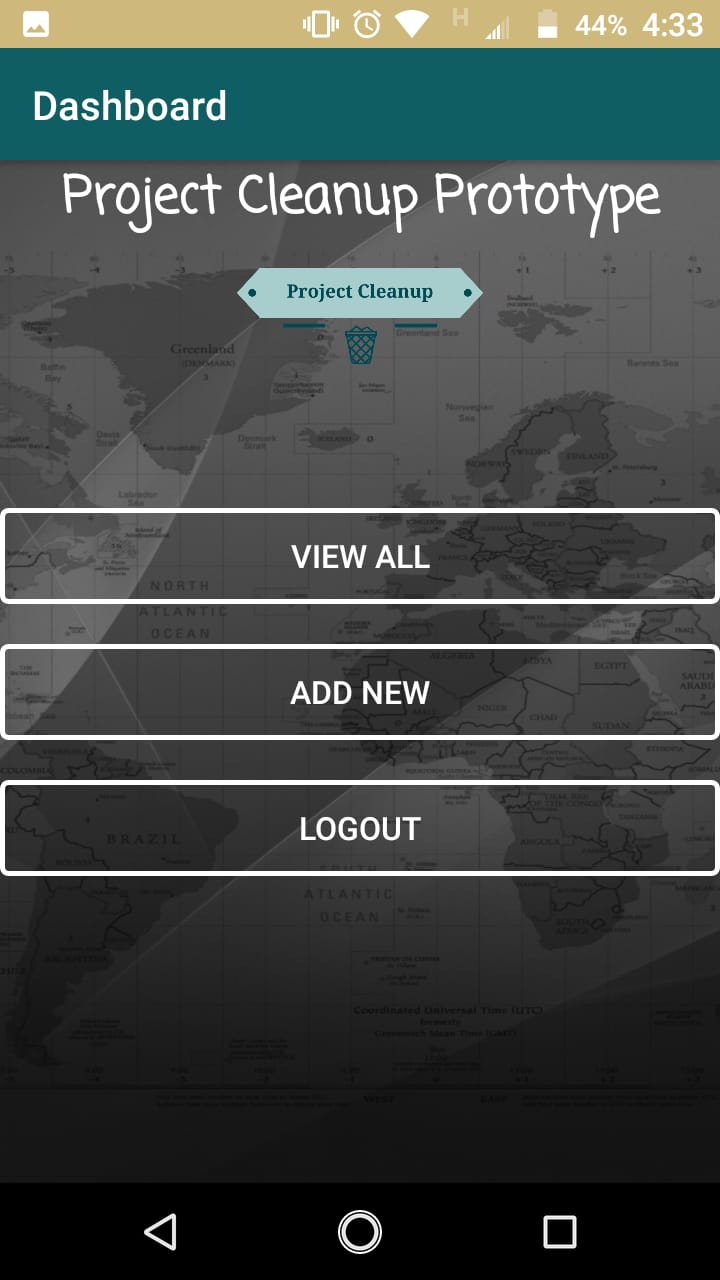
\includegraphics[scale=0.5]{images/3.png}
   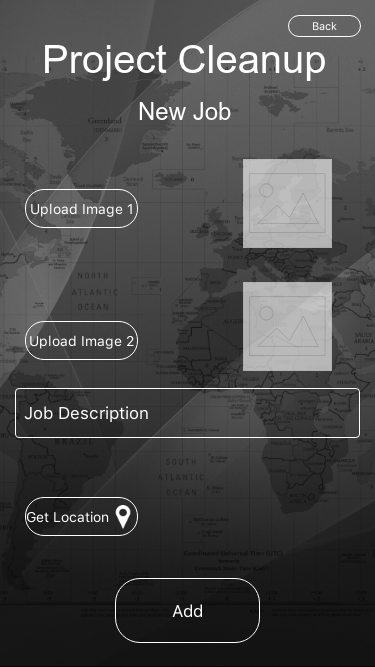
\includegraphics[scale=0.5]{images/4.png}
   
 
   \caption{User Panel}\label{fig:picture}
\end{figure}
After logging in, the user is presented with two options. A user can either add a new job or view the job list that is his/her previously submitted requests.\\
If the user clicks on add new job the app displays a new screen which asks the user to upload two images. User can also using the description box to add comments if he wants to. The user is then supposed to add the job which is a process of submitting his request. It is important to note that the location must be turned on in order to add the job.\\
The screens also consist of the "back" option.
If the User chooses the view jobs option and clicks on it then a new screen appears which shows the job list, that is previously submitted requests. This screen also consists of a back button.\\
\newpage
\begin{figure}[!hb]
   \centering

   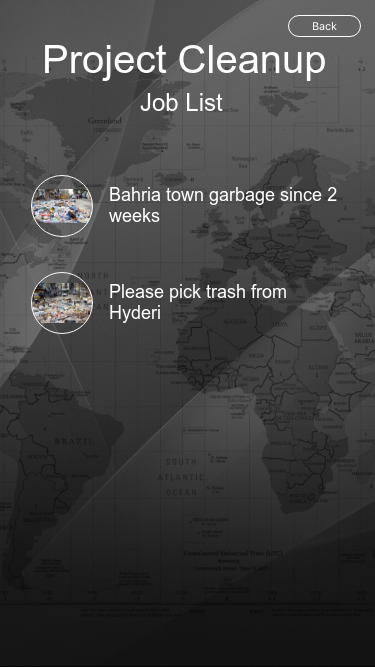
\includegraphics[scale=0.5]{images/5.png}
 
   
 
   \caption{User Panel}\label{fig:picture}
\end{figure}

\textbf{Admin Panel:}
The admin panel will be available on the web application. The web application will consist of an admin login screen. Through that screen the admin will be able to put in the ID and Password that he is assigned which will be authenticated and once that is done the admin will be able to log in.\\
\\
The admin will be able to do two tasks:\\
1)Admin will be able to view all the job requests that were submitted by the users.\\
2)The admin will also be able to view the route on the admin panel.

\newpage
\begin{figure}[!hb]
   \centering

   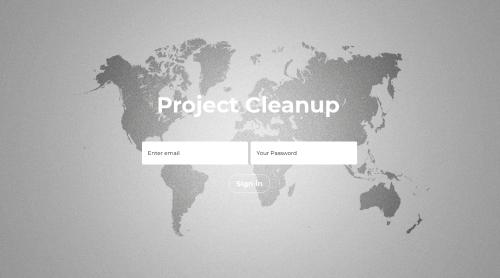
\includegraphics[scale=0.8]{images/6.png}
 \\
   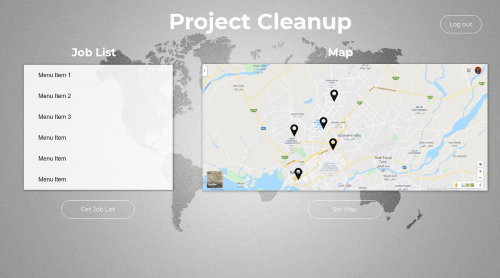
\includegraphics[scale=0.8]{images/7.png}
 
   \caption{Admin Panel}\label{fig:picture}
\end{figure}
\subsection{Application Program Interface (API)}
Our complete model will be able to take an image as input, identify segments of garbage and approximately quantify the volume of garbage,. Once our model has been made and is able to process data according to our requirements We will be uploading this model to a cloud server. AWS Lambda is one of the leading platforms for hosting models on cloud servers. 

In order for any client to use the model on the server we need a communication protocol. Once our model is on the cloud, AWS Lambda provides us with an application programming interface that can be easily connected with any interface of an application to use.
\newpage
\subsection{Hardware/Communication Interfaces}
This section describes the tools and technologies will be using for the different components of our project.\\
\textbf{Phone Application}:\\
For the user interface that is the front end we will be using ionic which is focused mainly on the look and feel and we think it will work best fro the UI interaction and the framework we would be using is React native. Our application will be for android users.\\
\textbf{Web Application}:\\
For the Web Application we will be using Javascript MVC Frameworks Angular JS/django node both of which are open source tools known for writing quick to write and powerful client-side web applications. We will also be using React, a javascript library, to make an interactive experience for the user.\\
\textbf{Cloud Server:}\\
We will be using AWS lambda as the cloud server AWS Lambda is one of the leading platforms for hosting models on cloud servers.AWS Lambda provides us with an application programming interface that can be easily connected with any interface of an application to use.\\
\textbf{Database:} \\
We will be exploring AWS and Firebase Database and use what works best for us.While we will be using MySQL which is a relational database management system based on SQL – Structured Query Language as backup.
\begin{figure}[!hb]
   \centering

   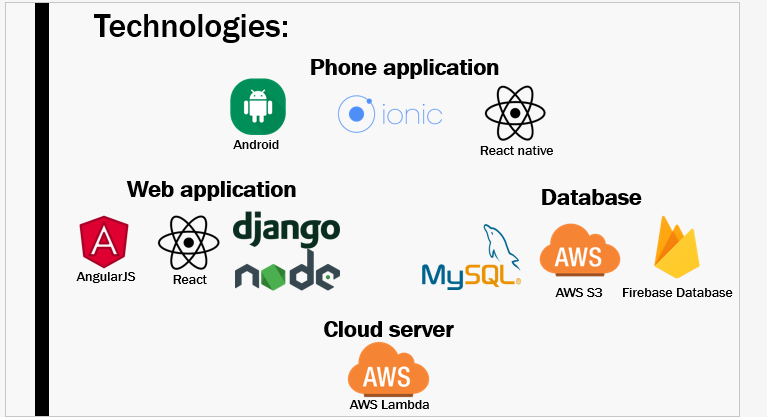
\includegraphics[scale=0.5]{images/Tech.PNG}

 
   \caption{Tools and Technologies}\label{fig:picture}
\end{figure}
\newpage
\section{Use Cases}
This section presents detailed use cases of our system.
\subsection{Admin:}
\begin{figure}[!hb]
   \centering

   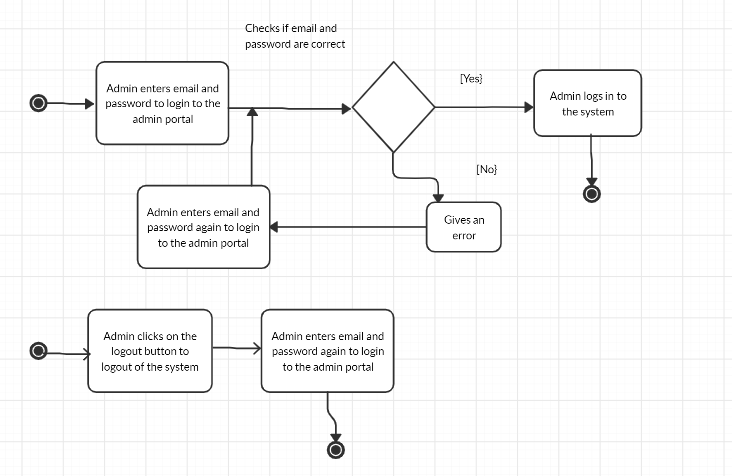
\includegraphics[scale=0.6]{images/Admin_1.PNG}

 

\end{figure}

\begin{figure}[!hb]
   \centering

   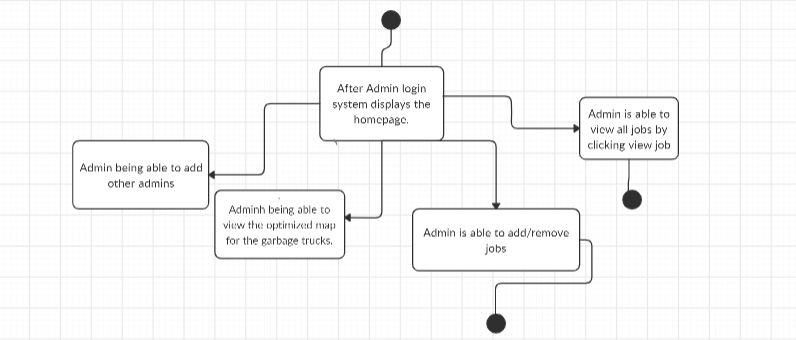
\includegraphics[scale=0.6]{images/Admin_3.PNG}
\end{figure}
\newpage
\subsection{User:}
\begin{figure}[!hb]
   \centering

   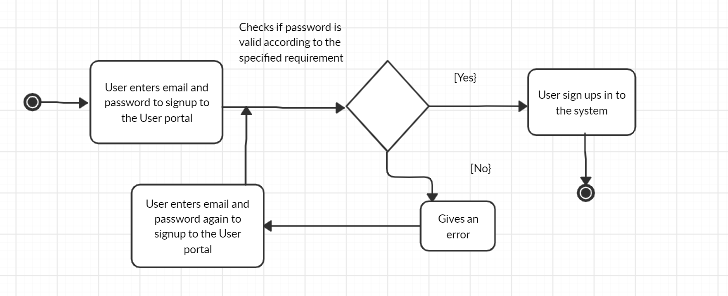
\includegraphics[scale=0.4]{images/User.PNG}
\end{figure}
\begin{figure}[!hb]
   \centering

   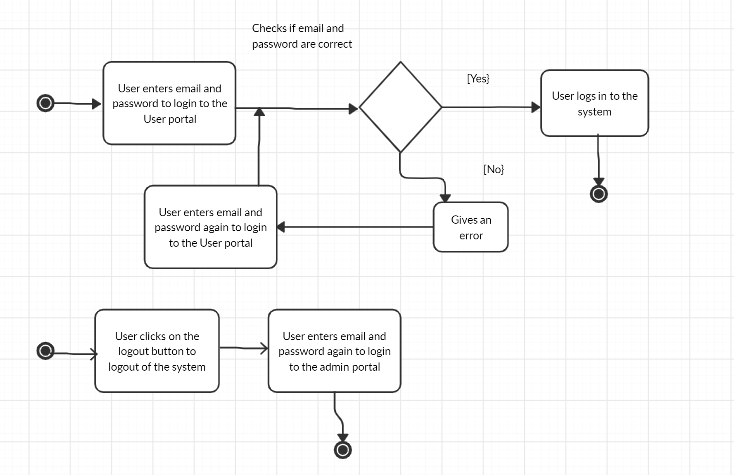
\includegraphics[scale=0.4]{images/User_1.PNG}
\end{figure}
\begin{figure}[!hb]
   \centering

   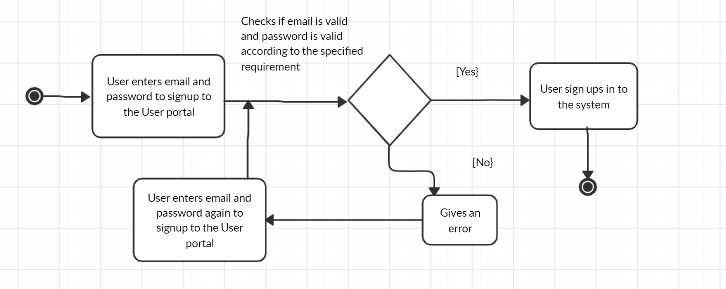
\includegraphics[scale=0.4]{images/User_2.PNG}
\end{figure}
\begin{figure}[!hb]
   \centering

   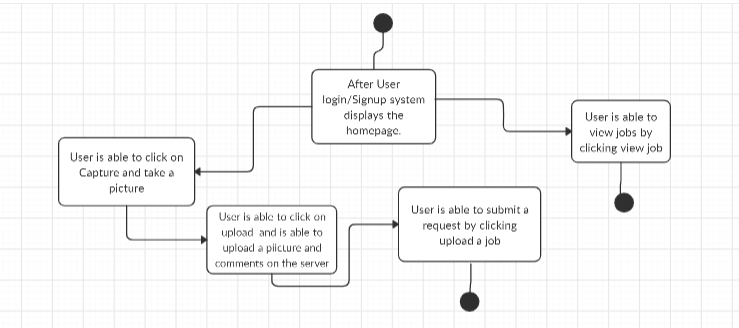
\includegraphics[scale=0.4]{images/User_3.PNG}
\end{figure}
\newpage
\subsection{System:}
The system activity diagram is divided into two parts: \\
The flow of the process and the decision making involved in the process. The flow of the process is from  the perspective of the user and the procedure explains the entire process happening behind the scenario that is after the user submits a request, the working of the system.

\begin{figure}[!hb]
   \centering

   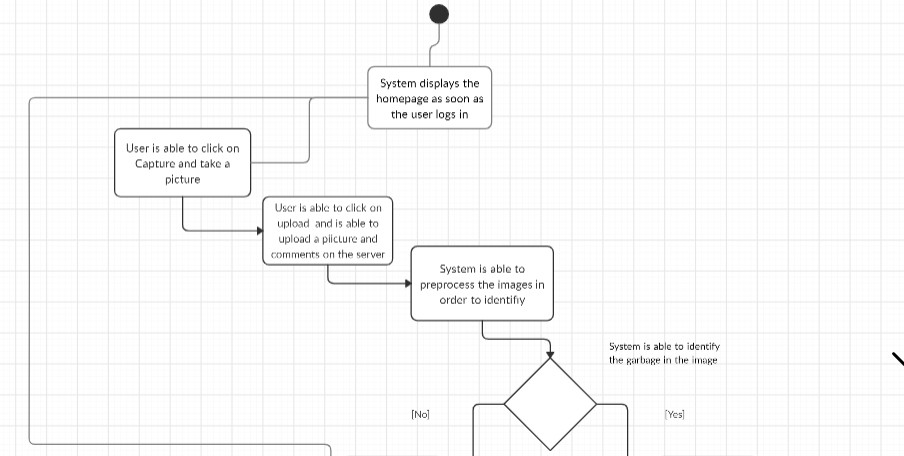
\includegraphics[scale=0.6]{images/UserSystem_1.PNG}
   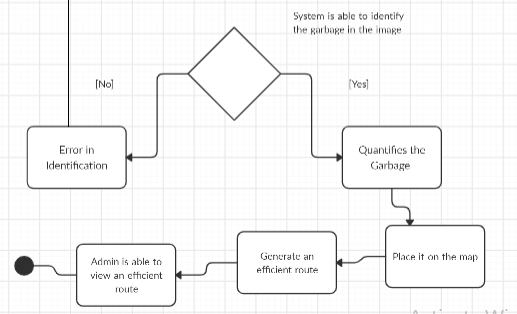
\includegraphics[scale=0.6]{images/UserSystem_2.PNG}
   
\end{figure}

\newpage
\section{Datasets}
One of the most important component of our project is the identification of the garbage and after our primary research we found out that work has been done on it and so we will be testing that out to incorporate it in our project. The application that works on the identification is called SpotGarbage.\\
We will be using their dataset which can be found at:\\
Garbage In Images (GINI) Dataset (https://github.com/spotgarbage/spotgarbage-GINI)\\
The dataset consists of categories of garbage and non-garbage, queries and non-queried images and  ambiguous annotated images. \\
\\
These categories further consist of garbage at various locations, litter, railway garbage, waste, street garbage, kitchen waste while non garbage images include buildings, chaos, streets, city, crowd, nature, texture, fruits and vegetables, earth+dust etc.\\
\\
We will also be creating our own dataset taking pictures of garbage from two different angles for the quantification component.

\begin{figure}[!hb]
   \centering

   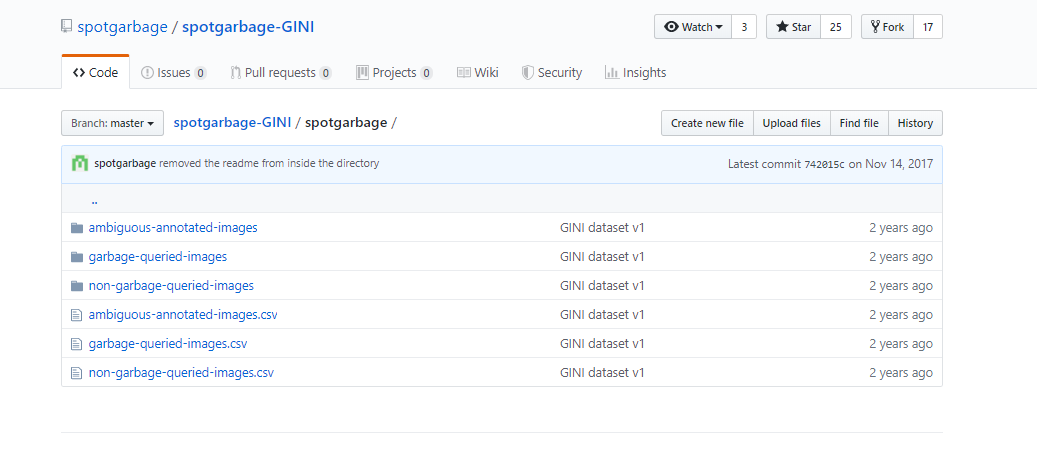
\includegraphics[scale=0.7]{images/Dataset.PNG}

 
   \caption{Dataset}\label{fig:picture}
\end{figure}
\newpage
\section{System Diagram}
This diagram gives a high-level view of the different components of our system and the interactions between them.\\
\textbf{User  app:}\\
Front end: ionic / Android / react native\\
Back end: Firebase Database\\
(Described in section 3.3.3)\\
\\
\textbf{Admin panel:}\\
Front end: Angular/ React\\
Back end: NodeJS / Django with Firebase Database\\
(Described in section 3.3.3)\\
\\
\textbf{Model Preprocessing:}\\
Python-OpenCV library:OpenCV is a Python library which is designed to solve computer vision problems.
\\
\textbf{Spotgarbage}:\\
Python-Caffe library:Caffe is good for fast training and testing, so if you want to experiment on different neural net architectures then it's a great choice because you don't even need to write code to design a neural net and things like fine tuning/transfer learning is extremely easy.\\
\\
Open-CV
\\
Pil:The Python Imaging Library (PIL) adds image processing capabilities to your Python interpreter.\\
\\
Numpy:Numpy is a general-purpose array-processing package. It provides a high-performance multidimensional array object, and tools for working with these arrays. It is the fundamental package for scientific computing with Python.\\
\\
\textbf{Quantification}: \\
Python image processing libraries\\
\\
\textbf{Cloud}:\\
AWS Lambda dependencies
\newpage
\textbf{System Diagram:}\\
\\
The system diagram is as follows:
\begin{figure}[!hb]
   \centering
   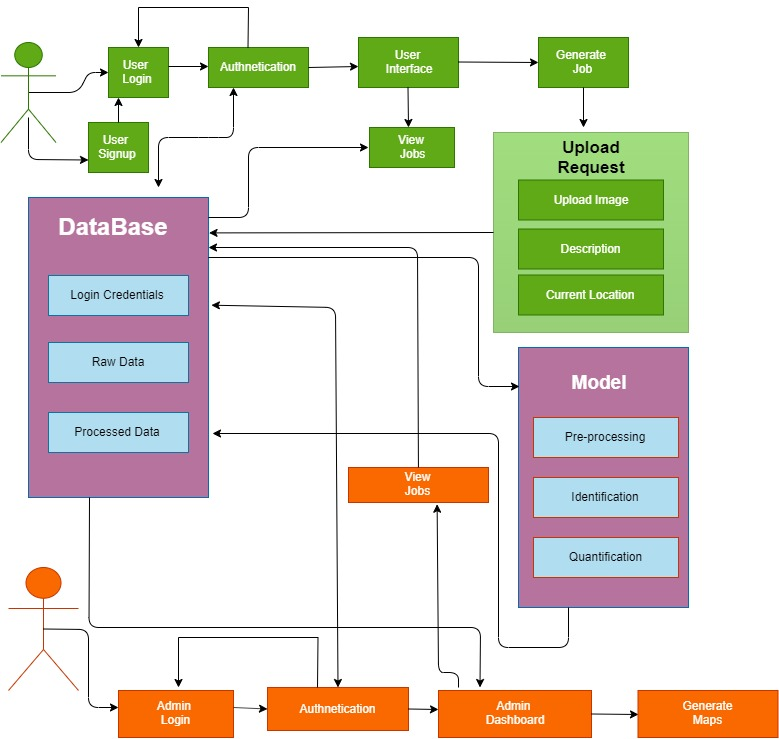
\includegraphics[scale=0.5]{images/8.jpeg}
   \caption{A Picture}\label{fig:picture}
\end{figure}

\chapter{Software Design 
Specification (SDS)}
\label{chap:sds}
This chapter provides important artifacts related to design of our project.

\section{Software Design}

This is a class UML Diagram which contain classes of the main actors alongside their attributes and their behaviors. There are 11 classes each having their own specific attributes and functions clearly defining the flow and functionality of the system.
\subsection{Classes}
\begin{enumerate}
    \item  User
    \item  Jobs
    \item  Routes
    \item  BaseUser
    \item  Sessions
    \item  Admin
    \item  Location
    \item  Images
    \item  Pre-Processing  (Static Class)
    \item GarbNetModel    (Static Class)
    \item Quantification  (Static Class)

\end{enumerate}


\newpage
\begin{figure}[!hb]
   \centering
   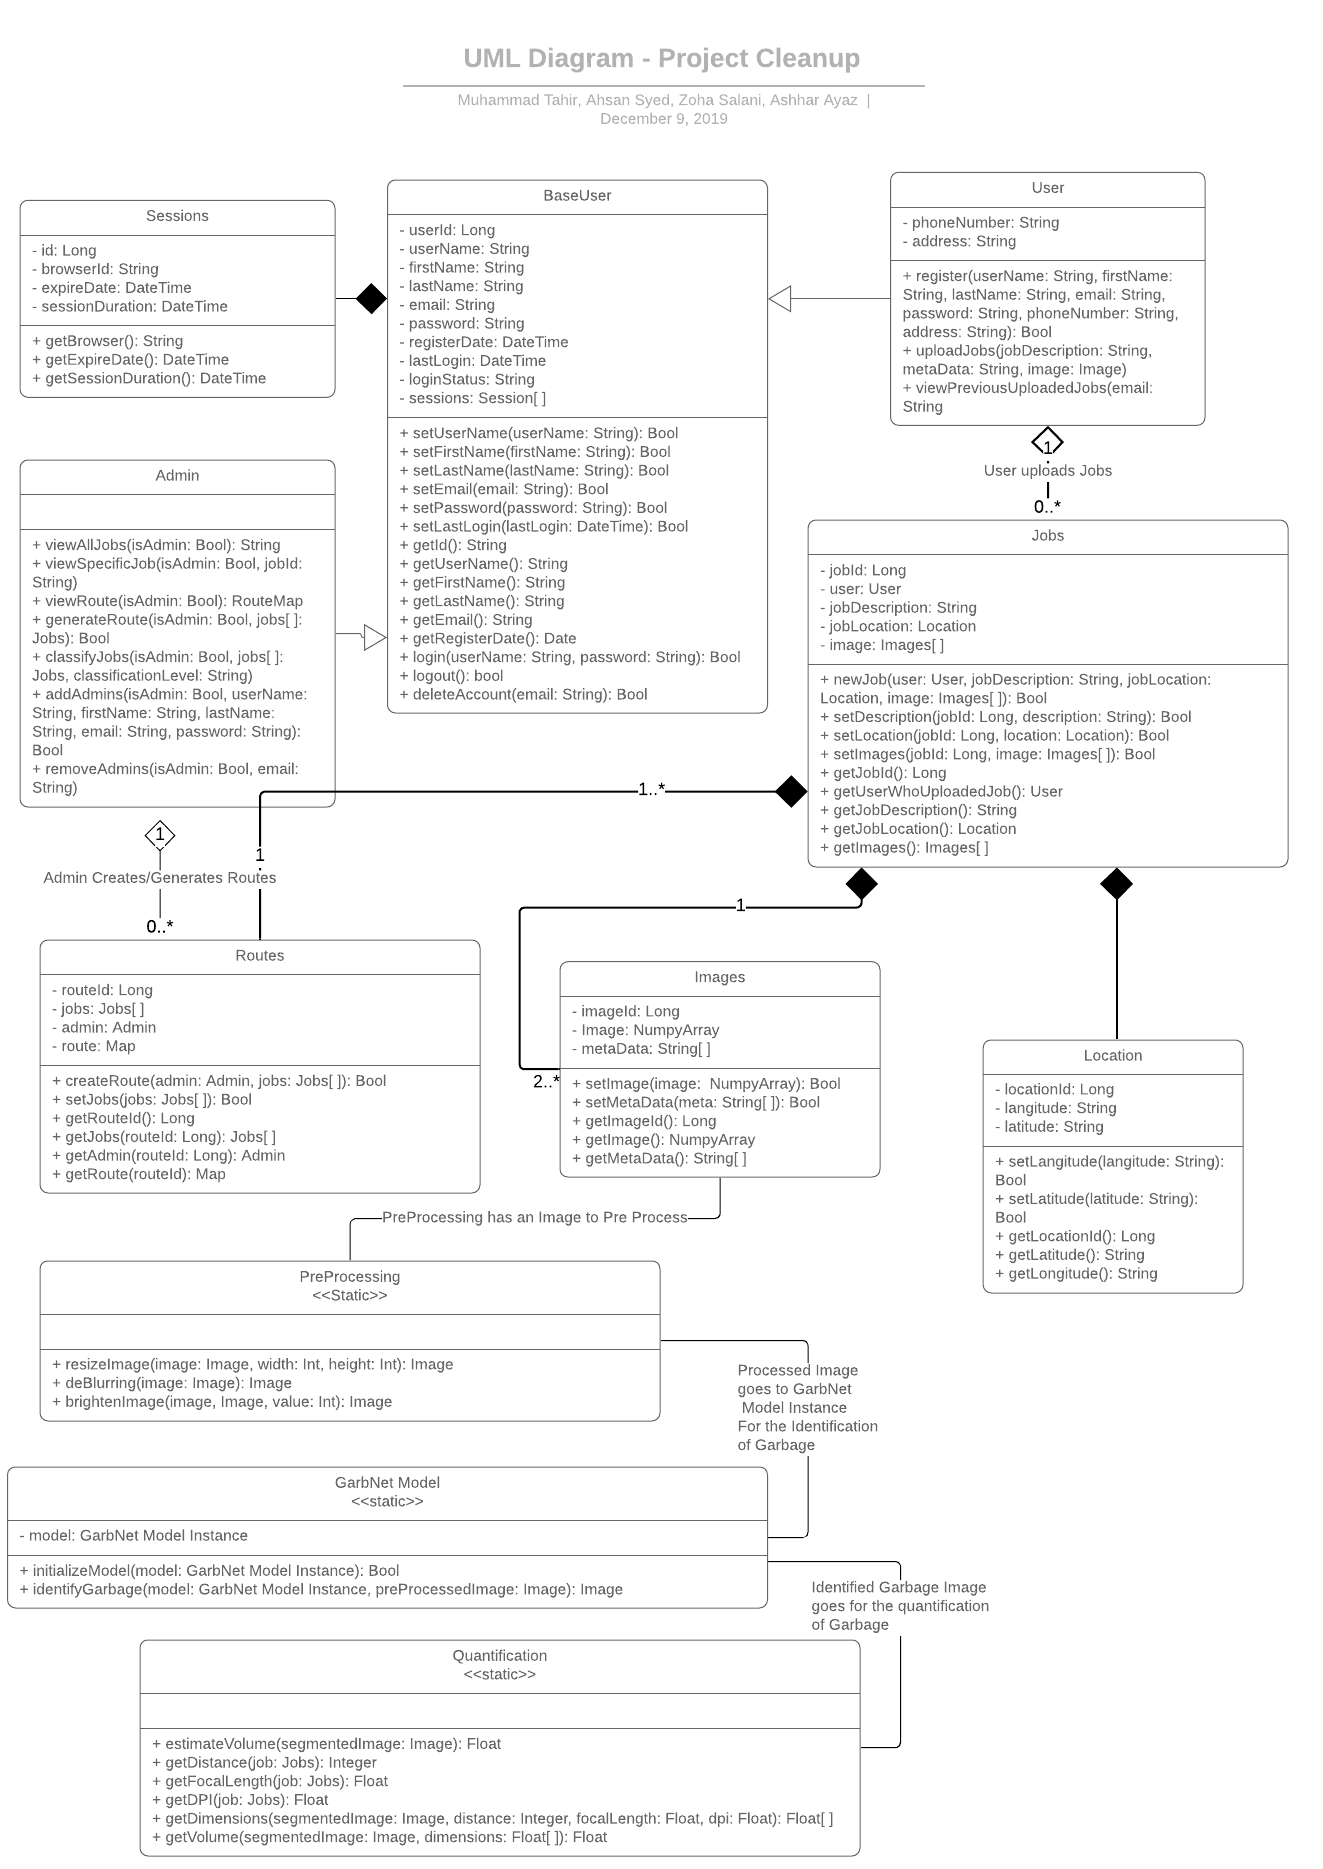
\includegraphics[scale=0.6]{images/UML.png}
   \caption{UML Diagram}\label{fig:picture}
\end{figure}

\subsection{UML Description}
Base User class refers to all the user classes that are accessing the system that is it includes both the User and the Admin but since they are separate entities (Actors) they will also have their own separate classes and will be inheriting from the parent class which in our case is the BaseUser. This particular class contains its particular attributes and functions that will remain the same for both the admin and the user entity. The relationship between the User class and the Admin class with the Base User is of generalization that is one element is a specialization of another general component. It may be substituted for it and is mostly used to represent inheritance. The Base User in this case is the Parent Class.\\
\\Now, Session Class having its defined attributes and functions is related to the BaseUser Class by the relation of Composition.The relationship is as such that if a composite object is deleted, all other objects associated with it are deleted. The composite object in this case is of the class BaseUser.\\
\\User Class having its own specific attributes and function is associated by aggregation relation with the Job Class that is a User can upload multiple Jobs. The relation is that of aggregation because the child class object can meaningfully, which in this case is Jobs, exist without the parent class object, unlike in composition.\\
\\Job Class having its specific attributes and functions is the composite for the Route, Images and Location Class that is if we delete the job, the route or image associated with that particular job will be deleted. The relationship is of composition.\\
\\Route Class is related to the admin by the relation of aggregation that is if we delete the admin the routes will still exist and if the Admin Class exist it can view all the routes generated.\\
\\The Image Class is associated with the the Pre-Processing Static Class as the latter accepts images and pre-processess. The Pre-Processed images are then passed into the GarbNet Model in order to identify garbage which is then passed to the Quantification Class. Here, the garbage is quantified, the volume is estimated and the value of Volume in Job class is updated for the Route Generation.


% Your report will contain ONE of the following 2 sections.
\newpage
\section{Data Design}

This section presents the structure of our database that caters to persistent data storage in our project. The structure is shown as a normalized data model for relational databases.
\subsection{ERD}
The ERD is the high-level conceptual diagram explaining the working of our project. This diagram shows the entities and the relationship of the entities stored in a database. The diagram will help explain the logical structure of the database.\\
\\The Entity Relationship Diagram for our database as follows:
\begin{figure}[!hb]
   \centering
   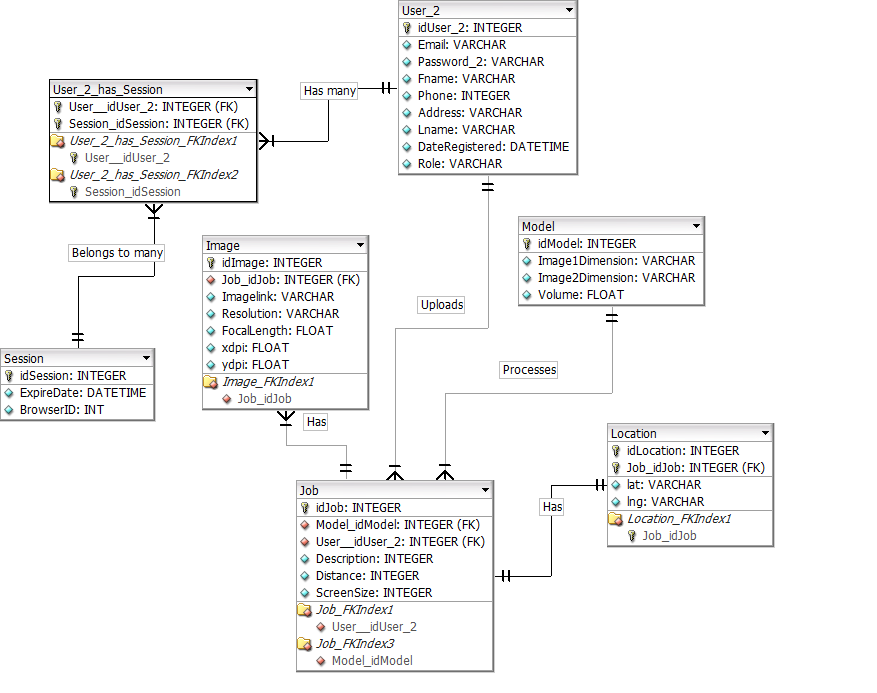
\includegraphics[scale=0.4]{images/ERD.png}
    \caption{Entity Relationship Diagram}\label{fig:picture}
\end{figure}
\newpage
Entities:\\
The strong entities in our relational diagram are as follows:\\
\textbf{1)User:}\\
\textbf{Primary Key:}UserID\\
\\
\textbf{2)Job:}\\
\textbf{Primary Key:} JobID\\
\textbf{Foreign Key:} AdminID\\
\textbf{Foreign Key:} UserID\\
\textbf{Foreign Key:} ModelID\\
\\
\textbf{3)Model:}\\
\textbf{Primary Key:} ModelID\\
\\
\textbf{3)Session:}\\
\textbf{Primary Key:} SessionID\\
\\
\textbf{4)Location:}\\
\textbf{Primary Key:} LocationID\\
\textbf{Foreign Key:} JobID\\
\\
\textbf{5)User has Session:}\\
\textbf{Primary Key:} UserID (FK)\\
\textbf{Primary Key:} SessionID (FK)\\
\\
\textbf{6)Admin:}\\
\textbf{Primary Key}: AdminID\\
\\
\textbf{7)Image:}\\
\textbf{Primary Key:} ImageID\\
\textbf{Foreign Key:} UserID\\
\\
Each entity has their own attributes that are specific to them. The entities also maintain a relationship between each other which is as follows:\\
\\
The User having login credentials and identifying fields, which are its specific attributes, is connected to the entity (Job) by a one to many relation that is one user can upload multiple jobs and can view the previous jobs. The User is also connected with the session entity which is a weak entity by a many to many relation since one session can have many users and one user can participate in various sessions.\\
\\
The Admin entity again with the login credentials and identifying fields is connected to the Job entity as one admin can view multiple jobs.\\
\\
The Model entity similarly is related to the Job entity by a many to one relationship as one model which exits for our application can process more than one jobs that are uploaded by the users.\\
\\
The Location Entity is related to the Job entity by a one to one relation since each Job will have a location of its own.\\
\\
Lastly, the image entity having its own attributes containing the image link and the image properties such as the resolution, focal length, location tag etc. is connected to the Job entity by having a one to may relation, that is a job can have multiple images but one specific image can belong to one and only one job only. The part where user can take multiple pictures is also catered as jobs contains the foreign key for the user entity.\\





 



\chapter{Experiments and Results}
\label{chap:results}
\section{Experiment - Identification of Garbage}
The first phase of the project was working on identifying garbage from an image. We tried to take an approach to train a Convolutional Neural Network to identify the garbage from an image and segment that part out. The first thing to do was to gather a large amount of labelled data (images of garbage) but before doing that we did our background research online to find any work done on this problem. Fortunately, we found a model already trained to identify garbage from the images. We decided to test that out and if that works, we could simply incorporate that model into our project.
\subsection{GarbNet Model}
The GarbNet Model was initialized on a pre-trained model, AlexNet, which is a model that is already trained on 1 million images of 1000-way object recognition. The architecture was customized to perform binary classification (is garbage, is not a garbage). More details about this model can be accessed by clicking on the heading $\-\>$ \href{https://dl.acm.org/doi/pdf/10.1145/2971648.2971731}{GarbNet Model - SpotGarbage}.
\section{Experiment - Quantification}
In this project, we tried different approaches for quantifying the volume of the garbage from an image. Those approaches are described in detail in the Literature Review (\ref{chap:lit}) section of the report. This section will briefly talk about all the methods, along with their advantages and disadvantages.
\subsection{3D Reconstruction from Multiple 2D Images}
This approach uses 2D images taken from different angles to reconstruct a 3D image. Susheel [5] proves that using 2D images from 8 different angles would improve the accuracy of our model to about 85 percent. This method seemed promising but given our target audience, the common man, this seemed a bit unrealistic. We came to the conclusion that not a lot of people would go around taking 8 different pictures of the same garbage dump from 8 different angles and therefore, we dropped this methodology and tried our luck with Depth Analysis and Stereoscopic Vision methodology.
\subsection{Depth Analysis and Stereoscopic Vision}
This approach uses two camera lenses spaced slightly apart to let the phone compare two images and piece together the depth of the object in stereo. With this methodology, using two cameras and their features, the accuracy of the model was promising (in theory) but we could not take this idea to its implementation because if we were to use this methodology in our project, then it would become a pre-requisite for the user of our app to have two cameras at their disposal, which was quite unrealistic. Therefore, we dropped this methodology and tried our luck with Dimension of Object - By Reference methodology. 
\subsection{Dimension of Object - (By Reference)}
This approach uses the camera parameters (DPI, Focal Length, etc.) of the device along with a reference object in the image with a known width and length. We tried this method, implemented it with our project and it was giving a very good result. However, one drawback of this method was that for every picture of the garbage dump that the user will upload on the app, they need to have a reference object (a human, a table, a chair, etc.) with a known width and height. Keeping in mind our target audience, the common man, this seemed unrealistic that all the images will have a reference object. Therefore, we dropped this methodology and tried our luck with Dimension of Object - By Distance methodology.
\subsection{Dimension of Object - (By Distance)}
The fundamental idea behind this approach is to still find the dimension of the object (garbage dump) from the image and using those dimensions, we can easily calculate the volume of the object. To get the dimensions of the object, we need to know the actual width and height of the object. We can get width if we have the height and vice versa. The methodology implemented uses camera parameters, the distance of the object from the camera (an approximate distance of the user from the garbage). 
\begin{figure}
    \centering
    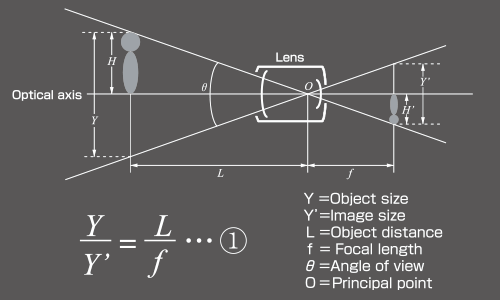
\includegraphics[scale=0.6]{images/dimensionDistance.png}
    \caption{Proportional Ratio of lens}
    \label{fig:lensRatio}
\end{figure}
\\
The equations used are as follows:
\begin{equation}
    \frac{Object Dimension}{Distance} = \frac{Object on Sensor Dimension}{Focal Length} 
\end{equation}
\begin{equation}
    Object Height = \frac{Object on Sensor Height * Distance}{Focal Length}
\end{equation}
where Object Height (m) - value to find,\\
Object on Sensor Height (mm) - get this in terms of pixels,\\
Distance (m) - User will input this hyperparameter,\\
and Focal Length (mm) - can be obtained by camera.\\
As mentioned above, we already are getting focal length and distance and we can simply put in the values in the equation and get the result. One drawback of this approach was that, we could only extract height from image in terms of pixels. We needed the height on sensor in terms of mm (the actual distance). One method that we tried was converting pixels into mm via dots per inch/ pixels per inch.  We need height in terms of \textbf{mm} and we are getting in terms of \textbf{pixels}. The equation below will show you the reasoning and mathematics behind it. 
\begin{equation}
    1 Pixel = \frac{25.5 mm}{Dots/Pixel Per Inch}
\end{equation}
How many pixels are on 1 inch of screen? We can get that using the equation below:
\begin{equation}
    Dots/Pixels per Inch = \frac{Pixel Diagonal}{Screen Diagonal}
\end{equation}
where as we can get xdpi and ydpi from the android application, and height and width in pixels, and height and width of phone screen.\\
However, the resulting height of the garbage in terms of mm was being incorrectly calculated using this methodology. The reason was that we were calculating in terms of dots per inch but that was also dependent on sensor of the camera. So we needed to focus on getting the the dimensions of sensor. Only then can we effectively convert the image from pixels to mm. Therefore, we had to stop using dpi/ppi and find another method to convert from pixels to mm. One method we tried was using Field of View of the lens. It was the angle at which our camera works. The below figure will give you an idea of how it is used:\\
\begin{figure}
    \centering
    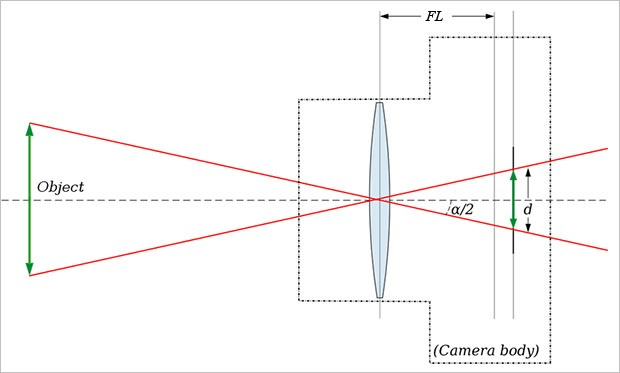
\includegraphics[scale=0.5]{images/fov.jpeg}
    \caption{FOV relation to the Image}
    \label{fig:fov}
\end{figure}
\\
Using the properties of ratios, we can tell that through the camera angle (Field of View), the image is projected on to the sensor. Using this information and trigonometry, we can get the width and height of the garbage using either horizontal angle or vertical angle. The equation, in either case, would be as follows:
\begin{equation}
    Sensor Width = tan(horizontal angle/2) * 2 * Focal Length   
\end{equation}
Once we have the sensor width, we can simply calculate the width of garbage in mm using the following equation:
\begin{equation}
    Width of Garbage (mm) = \frac{Width of Garbage in Pixels * Sensor Width}{Width of Entire Image}
\end{equation}
Once we get the width using the horizontal angle, we can then simply use the ratios between the original width and pixel width to find the original height of the garbage using the following equation:
\begin{equation}
    Original Height (mm) = \frac{Original Width * Sensor Height}{Sensor Width}
\end{equation}
Now, once we have the height and width of the garbage from two different images, we can then use them to find the volume of the garbage.
\section{Optimizations}
Once we had the volume, we realised that the volume is a bit of an overestimate of the actual volume of the object. This was due to the fact that spotgarbage (the GarbNet model) always produces an overestimate bounding box of the garbage dump. Taking that into account, we tried to find ways to reduce that effect of overestimating and in return, optimizing our model. One method that we tried was that we tried multiple objects with known bounding boxes and compared them with the output of the spotgarbage. This way, we found an average percentage error that the GarbNet model was making and how much it was overestimating. Using the findings from this experiment, we put an underestimating multiplying factor to the final bounding box and found that it gave much better results than the previous implementation. Once we got the bounding boxes of our object (garbage patch) at hand, we calculate the volume of those bounding boxes within which our garbage is encapsulated. We use known volumes of regular shapes to better our calculation results of the irregular shapes. We use the shape of the pyramid and cube with its known volume to make a sense of how  our final calculated volume could come as close to the actual volume of our irregular shaped garbage.
\section{Result}
The resulting product of our project is an Android Mobile Application that communicates with the Web Admin Portal through third party Cloud Storage and Services.
\subsection{Android Mobile Application}
The application was developed on Android Studio that uses java as its back-end language, and xml as its front-end and linking language. The implementation and design of the Android Mobile Application is displayed in the SDS section (\ref{chap:sds}) above.
\subsection{Cloud Storage and Services}
Early on in the development stage, we focused on Amazon Web Services platform for our cloud related queries. At the same time, we also explored Google Cloud Platform as a backup plan in case AWS doesn't work out. Comparing those two platforms and its user interface and friendliness, we switched to Google Cloud Platform because it was much more easier to understand and navigate. More information about this can be found in the SDS section (\ref{chap:sds}) above.
\subsection{Database - Google Firebase}
As mentioned above, we decided on using Google Cloud Platform and thus used Google's mobile application development platform (Firebase) as our real time database for the project.
\subsection{Web Admin Portal}
Web Admin portal was developed using website development tools (html, javascript, css, etc.). It's a portal that uses the Google Cloud Platform to communicate with the mobile application.  More information about this can be found in the SDS section (\ref{chap:sds}) above.

\subsection{Integration}
As mentioned above, we had three stand alone resulting products of our project: Mobile App, Cloud Model, Web App. Integration deals with integrating the three stand alone parts into one complete final product known as Project Cleanup. \\
\\
The way we integrated that was that we developed a python script that listens onto the bucket in the Firebase Real Time Database and whenever a new job is posted from the mobile app, the listener gets triggered and the script starts executing. The basic overflow of the script is as follows: The job posted has some images with it that are stored in firebase. The script downloads those images from firebase to its base location on Google Cloud Storage and passes it through the GarbNet model to segment out the garbage in the image.\\
\\
Once GarbNet recognizes the garbage, the segmented part is then passed onto the Quantification model that calculates the volume of the garbage in the images and update the volume's value back on the firebase, which can later be accessed by the Web Admin App to display the information about each job, their location, and the approximate volume of garbage present there.\\
\\
There were some challenges that we faced along the way. One challenge was integrating firebase with javascript, it was very difficult to do that but in the end, it got resolved. Another challenge was making the flow of the final product as smooth as possible with minimum delay in between.\\
\\
Having said all that, the project is fully functional with the Mobile App, Web App and the Cloud Script ready. The script hosted on Google Cloud runs 24/7 and listens for job posting through the mobile app.

\chapter{Conclusion and Future Work}
\label{chap:outro}
\section{Conclusion}

There are two major parts of our entire system. The first part is the SaaS (Software as a service) which enables two way communication between end users and administrations. The end user only needs to have the easy-to-use application on their mobile phones. The database itself is on cloud, which works on records in real time. \\
\\
The second part is that of our cloud model that is responsible for calculating a volume of an irregular shape after taking images as input. Once an end user via their mobile app uploads a job, our cloud model automatically fetches the data from the database and performs some operations on it. There are two major responsibilities that the model has. One is to perform some preprocessing and identify garbage and the second is to compute the volume.\\
\\
The identification is done via an already trained model called ‘SpotGarbage’, which used a Conventional Neural Network (CNN) on a garbage dataset and successfully learned to detect the patterns of garbage from an image.  \\
Once identification part is done, then we move towards the processing of the volume of the garbage. This is done using an approach based on similar triangle ratios.  Once we get the volume, we also optimize the result by utilizing the volumes of known shapes and incorporating that in the volume of the irregular shape of our garbage.\\
\\
Finally, once the volume has been calculated, it is pushed back to the database, which can be seen on the admin panel. The admin panel is able to see all the jobs each user has posted as well as their location and volume (of garbage). The admin can plan a route accordingly to the positions of the garbage for truck drivers efficiently in this manner. Once a the garbage has been collected, an admin can mark its status as done which can also be seen on the users end when they look at the lists of job they uploaded.


\section{Future Work}

These are some of the future potentials of our system:
\begin{enumerate}
    \item The application of our project can be further enhanced if local administration or different NGOs implement this which working on the waste management sector.
 
    \item The route generation can be further enhanced for individual truck drivers who will be responsible in collecting the garbage from the specific locations. 

    \item Once our system gets enough data gathered of garbage dumps around the city, it can use this data to actually pin point how much garbage is calculated in which area which can effectively improve waste management

    \item Our cloud model is the capability to calculate the volume of any irregular shape if that shape can be identified in a bounding box. This can be further applied in various scenarios like calculating volumes of containers, pile of clothes, pile of rocks etc.
\end{enumerate}

\begin{appendices}

\titleformat{\chapter}[hang]{\bf\huge}{Appendix \thechapter.}{2pc}{}
% \titleformat{\chapter}[hang]{\bf\huge}{\thechapter.}{2pc}{}

  
% This appendix is optional.
\chapter{More Math}
Here is the math used in the process:\\
\\
The links below talks more about the quantification equations used in our math in the paper above. 
Alternately, the link to it is as follows:\\
\href{https://petapixel.com/2013/06/15/a-mathematical-look-at-focal-length-and-crop-factor/}{Link 1}\\
\href{https://www.scantips.com/lights/fieldofviewmath.html}{Link 2}
\\
\\
\begin{figure}[!hb]
   

   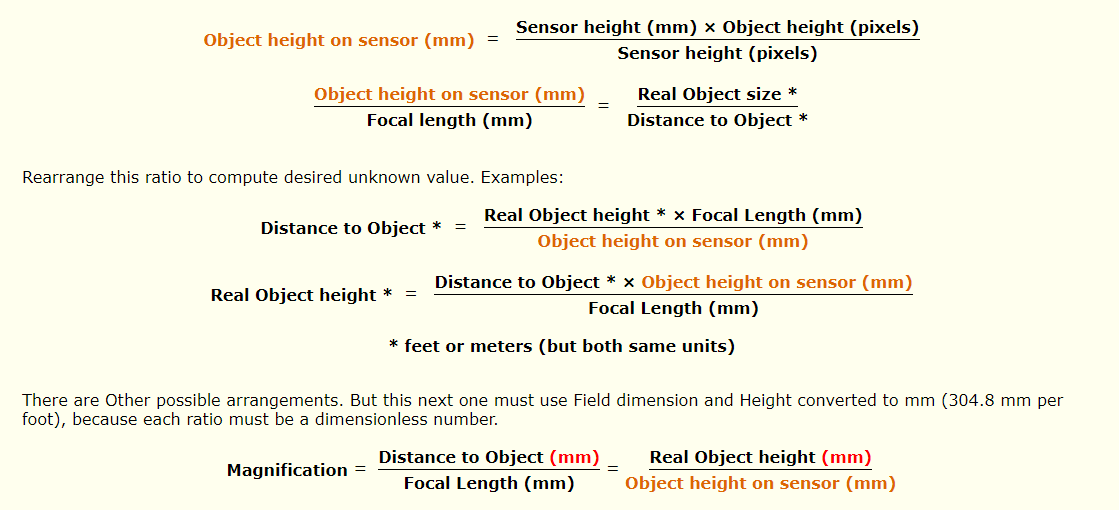
\includegraphics[scale=0.5]{images/MATH.PNG}

 
   \caption{Equations used in Quantification}\label{fig:GINIdataset}
\end{figure}


% This appendix is required if the data set is not fully described in the main text.
\chapter{Data}

Since we could not collect our own data due to COVID-19, here is the Dataset we used:\\
https://github.com/spotgarbage/spotgarbage-GINI.
\href{https://github.com/spotgarbage/spotgarbage-GINI}{GINI Dataset on Github} 

\begin{figure}[!hb]
   
    \centering
        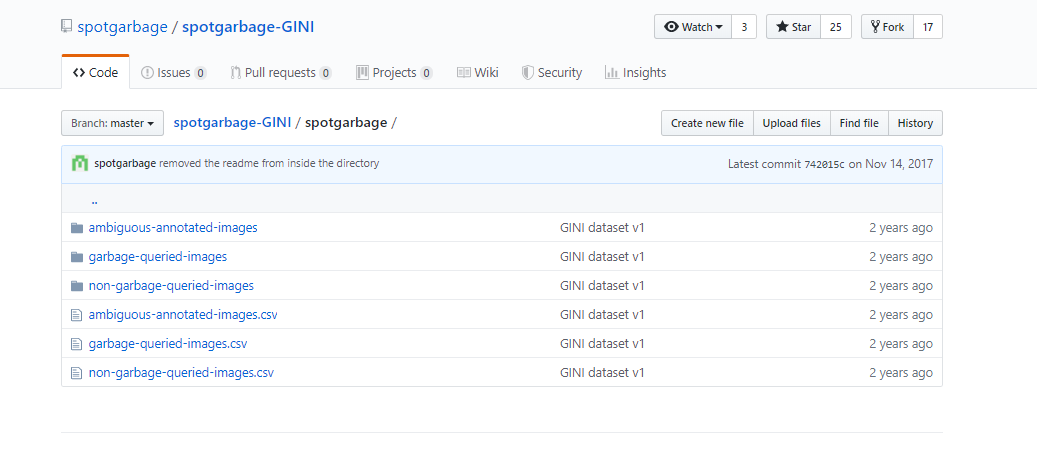
\includegraphics[scale=0.7]{images/Dataset.PNG}

 
   \caption{Dataset}\label{fig:GINIdataset}
\end{figure}

% This appendix is required if the code is not fully described in the main text.
\chapter{Code}
Here is our code:

% inspired by https://xkcd.com/221/
\begin{figure}[!hb]
    \centering
    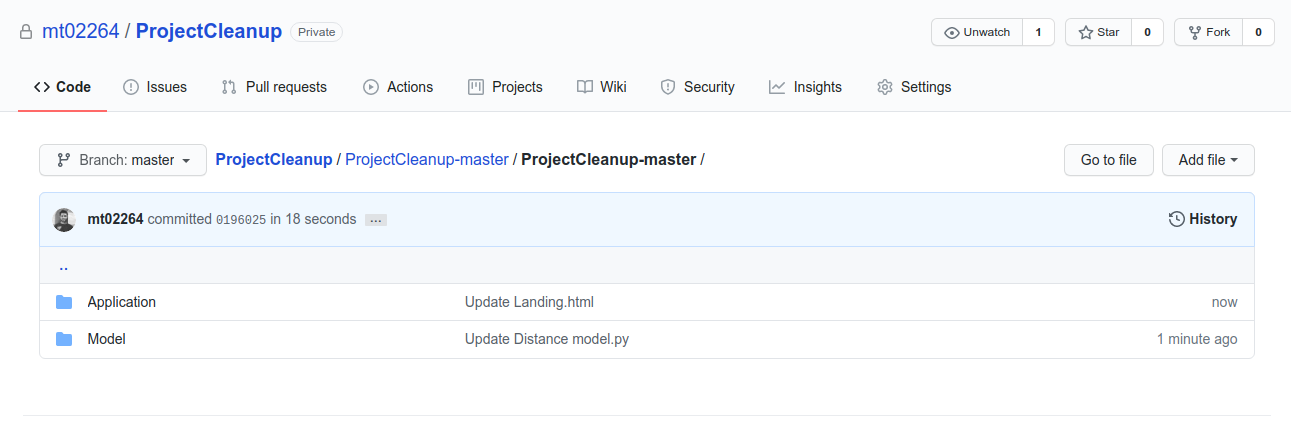
\includegraphics[scale=0.35]{images/ProjectsCleanup.png}
    \caption{Snippet of our Github Repository}
    \label{fig:GithubProject}
\end{figure}


Alternately:\\
Our code can be found at this  \href{https://github.com/mt02264/ProjectCleanup}{Github Repository (mt02264)}

%%% Local Variables:
%%% mode: latex
%%% TeX-master: "../report"
%%% End:

\end{appendices}

% Print the bibliography with a ToC entry and titled, "References".
\printbibliography[heading=bibintoc,title={References}]

\end{document}

%%% Local Variables:
%%% mode: latex
%%% TeX-master: t
%%% End:
